\documentclass[a4paper, 12pt]{extreport}
\usepackage{xcolor}
\usepackage{color}

\usepackage[unicode]{hyperref}
\usepackage[nottoc,numbib]{tocbibind}
\hypersetup{colorlinks=true, urlcolor=black, linkcolor=black, unicode=true}
\usepackage[utf8]{inputenc}
\usepackage[T5]{fontenc}      % Crucial for Vietnamese characters
\usepackage[english]{babel} % nếu viết bằng tiếng Việt thì bỏ dấu % đi
\usepackage{fancybox}
% \usepackage[utf8]{inputenc} % Hỗ trợ tiếng Việt
% \usepackage[vietnamese]{babel} % Hỗ trợ tiếng Việt
\usepackage{minted}
\usepackage{xurl}
\usepackage{frame}
\usepackage{framed}
\usepackage{graphicx}
\usepackage{indentfirst}
\usepackage{comment}
\usepackage[skip=10pt plus1pt, indent=25pt]{parskip}
\usepackage[a4paper, left=25mm, right=20mm, top=25mm, bottom=25mm]{geometry}
\usepackage{tikz}
\usepackage{subfig}
\usepackage{pgfplots}
\usepackage[justification=centering]{caption}
\usepackage{titlesec}    
% \usepackage{times}
\usepackage{amssymb}
\usepackage{amsmath}
\usepackage{booktabs}  % Để kẻ dòng đẹp (\toprule, \midrule, \bottomrule)
\usepackage{tabularx}  % Để tự động xuống dòng và căn chỉnh độ rộng cột
\usepackage{mathpple}
\usepackage{listings}
\usepackage{scrextend}

\definecolor{dkgreen}{rgb}{0,0.6,0}
\definecolor{gray}{rgb}{0.5,0.5,0.5}
\definecolor{mauve}{rgb}{0.58,0,0.82}
\lstset{frame=tb,
  language=C++,
  aboveskip=3mm,
  belowskip=1mm,
  showstringspaces=false,
  columns=flexible,
  basicstyle={\small\ttfamily},
  numbers=none,
  numberstyle=\tiny\color{gray},
  keywordstyle=\color{blue},
  commentstyle=\color{dkgreen},
  stringstyle=\color{mauve},
  breaklines=true,
  breakatwhitespace=true,
  tabsize=3
}

\usepackage[backend=bibtex,style=ieee]{biblatex} 
\addbibresource{references}
\pgfplotsset{compat=1.18}
\begin{document}
\thispagestyle{empty}

\begin{center}

% University name
{\Large \textbf{HANOI UNIVERSITY OF SCIENCE AND TECHNOLOGY}}\\[4pt]
{\large School of Information and Communications Technology}\\[1pt]

\rule{12cm}{0.4pt}\\[1.5cm]

% Logo

\includegraphics[width=4cm]{logo-hust.png}\\[1.8cm]

% Title
{\fontsize{32pt}{1}\selectfont \textbf{PROJECT REPORT}}\\[0.4cm]
{\fontsize{20pt}{1}\selectfont DEEP LEARNING -- IT4653}\\[0.8cm]
{\fontsize{18pt}{1}\selectfont \textbf{Project}\\
\fontsize{15pt}{1}\selectfont \textbf{MovieRAG: Enhanced System with Movie Knowledge Graph}}\\[1.8cm]

% Student info
\begin{table}[h]
    \centering
    \renewcommand{\arraystretch}{1.3}
    % Thay đổi cột cuối thành X để tabularx hoạt động
    \begin{tabularx}{\textwidth}{|c|l|c|X|} 
        \hline
        \textbf{STT} & \textbf{Họ và Tên} & \textbf{MSSV} & \textbf{Email} \\
        \hline
        1 &  Nguyễn Quốc Bảo Long  & 20230045 & long.nqb230045@sis.hust.edu.vn \\
        \hline
        2 & Nguyễn Đình Lâm Phúc   & 20235193  & phuc.ndl235193@sis.hust.edu.vn \\
        \hline
        3 & Nguyễn Khánh Hưng  & 20235100  & hung.nk235100@sis.hust.edu.vn \\
        \hline
        4 & Trần Nguyên Thành    & 20235224  & thanh.tn235224@sis.hust.edu.vn \\
        \hline
    \end{tabularx}
\end{table}
% Supervisors
{\Large \textbf{Supervisors}}\\[6pt]
{\large \textbf{Assoc Prof. Nguyễn Hồng Quang}}\\
{\textbf{Class: }}
\vfill
{\large Ha Noi, \number\year}

\end{center}

\setcounter{tocdepth}{1}
\newpage

\begin{abstract}
Large Language Models (LLMs) have demonstrated remarkable capabilities in natural language understanding; however, they remain prone to hallucinations and lack up-to-date knowledge in specialized domains. While Retrieval-Augmented Generation (RAG) \cite{lewis2020rag}  mitigates these issues by retrieving relevant context, traditional vector-based approaches often treat data snippets in isolation, failing to capture the complex structural dependencies essential for reasoning. This paper presents the design and implementation of a movie-domain chatbot leveraging GraphRAG (Retrieval-Augmented Generation with Graphs) to address these limitations. Unlike naive RAG systems, our approach models the underlying movie database as a Knowledge Graph (KG) \cite{han2025retrievalaugmentedgenerationgraphsgraphrag} , explicitly representing relationships between heterogeneous entities such as actors, directors, and genres. By integrating graph traversal algorithms with semantic retrieval, the system identifies and retrieves relevant subgraphs, providing the LLM with structured, topologically rich context for answer generation. Experimental evaluations demonstrate that the GraphRAG-based architecture \cite{han2025retrievalaugmentedgenerationgraphsgraphrag} significantly outperforms baseline methods in handling multi-hop queries and relational reasoning tasks. This study highlights the efficacy of combining symbolic graph structures with neural language models to build more robust and context-aware conversational agents.
    
\end{abstract}
\tableofcontents

\newpage

\chapter{Introduction}

\section{Motivation}
The unprecedented evolution of Large Language Models (LLMs) has fundamentally redefined the boundaries of Natural Language Processing. These models have become ubiquitous, endowing artificial agents with the capacity to comprehend and generate human-like text with remarkable fluency \cite{devlin-etal-2019-bert, touvron2023llama}. In the context of the entertainment industry, specifically movie recommendation and discovery, this advancement offers a significant opportunity to transform how users interact with cinematic databases. Users no longer seek simple keyword-based results; they demand intelligent agents capable of understanding complex, context-rich queries such as identifying artistic collaborations or exploring thematic similarities across film franchises.

However, the movie domain is characterized by high \textit{relational density}. Entities such as actors, directors, genres, and production studios are not isolated data points but are inextricably linked through a complex web of artistic and professional collaborations. To fully leverage the potential of LLMs in this domain, there is a critical need for a framework that can not only retrieve information but also comprehend the \textbf{topological structure} of these relationships. This necessitates a paradigm shift towards Retrieval-Augmented Generation with Graphs (GraphRAG)  \cite{han2025retrievalaugmentedgenerationgraphsgraphrag}, which utilizes Knowledge Graphs to preserve the semantic context necessary for answering sophisticated user queries.

\section{Problem Statement}
Despite their linguistic proficiency, deploying LLMs for specialized domain tasks presents significant challenges. The first intrinsic limitation is the phenomenon of hallucination \cite{maynez-etal-2020-faithfulness}, where the model generates plausible but factually incorrect assertions. Additionally, LLMs are constrained by their static training data, rendering them incapable of accessing real-time information or private knowledge bases developed after their training cutoff \cite{lewis2020rag}.

While conventional Retrieval-Augmented Generation (RAG) frameworks  \cite{lewis2020rag} attempt to mitigate these issues by indexing external knowledge within a vector database, they encounter critical bottlenecks:

\begin{enumerate}
    \item \textbf{Loss of Structural Relationships:} Conventional RAG processes documents by partitioning them into discrete segments and encoding them into high-dimensional vectors. This "naive" vector-based approach treats data points as independent entities in a latent space, inadvertently discarding the explicit structural dependencies that exist between them.
    
    \item \textbf{Inability to Handle Multi-hop Queries:} By flattening rich information into isolated vectors, vector-based systems struggle to synthesize information that requires traversing multiple logical steps. For instance, a query like \textit{"Find movies directed by Christopher Nolan that feature actors who also played in Marvel films"} requires understanding the interconnected nature of entities, which is often beyond the reach of semantic similarity metrics like cosine similarity alone \cite{han2025retrievalaugmentedgenerationgraphsgraphrag}.
\end{enumerate}

Therefore, the core problem this research addresses is the inadequacy of flat, vector-based retrieval methods in capturing the complex, interlinked semantics of the movie domain, and the need for a holistic GraphRAG \cite{han2025retrievalaugmentedgenerationgraphsgraphrag} approach to enable accurate, context-aware reasoning.
\section{Project Objectives}
The primary goal of this project is to attempt to design and implement a \textbf{Graph Retrieval-Augmented Generation (GraphRAG)} \cite{han2025retrievalaugmentedgenerationgraphsgraphrag} system tailored for the movie domain. This system aims to overcome the limitations of flat vector-based retrieval by integrating structured knowledge representations with the generative capabilities of Large Language Models.

To achieve this main goal, the project focuses on the following specific objectives:

\begin{enumerate}
    \item \textbf{Construction of a Movie Knowledge Graph (MKG):} 
    To design a comprehensive ontology and construct a Knowledge Graph using \textbf{Neo4j} \cite{neo4j}, a widely-used tool for graph-based tasks. This involves modeling complex cinematic entities (e.g., \textit{Director, Actor, Genre, Movie}) and their semantic relationships (e.g., \textit{`DIRECTED\_BY`, `ACTED\_IN`, `SEQUEL\_OF`}) to preserve the topological structure of the data that is typically lost in vector-based approaches.

    \item \textbf{Development of a Graph-Enhanced Retrieval Pipeline:} 
    To implement a retrieval mechanism that goes beyond simple semantic similarity \cite{10.1145/361219.361220,reimers2019sentencebert}. The system will utilize graph traversal algorithms (such as multi-hop reasoning) to extract interconnected subgraphs relevant to user queries, thereby addressing complex questions that require logical reasoning across multiple entities (e.g., finding common collaborators between two directors).

    \item \textbf{Integration of Neuro-Symbolic AI:} 
    To create a seamless integration between the symbolic reasoning of the Knowledge Graph and the probabilistic generation of LLMs (\textbf{Google Gemini}). This involves designing prompt templates that effectively utilize the retrieved graph context to ground the LLM's responses, minimizing hallucinations and ensuring factual accuracy.

    \item \textbf{Empirical Evaluation and Comparison:} 
    To evaluate the performance of the proposed GraphRAG framework against a baseline "Naive" RAG system (Vector-only). The evaluation will focus on key metrics such as answer faithfulness, relevance, and the ability to correctly handle multi-hop queries.
\end{enumerate}
\section{Scope and Limitations}

\subsubsection{Scope of the Project}
This research focuses on the development of a backend-heavy retrieval system and a user-facing chatbot interface. The specific boundaries of the project are defined as follows:

\begin{itemize}
    \item[] \textbf{Data Coverage:} The system utilizes the \textbf{TMDB (The Movie Database)} Dataset, where information of thousands of movies will be collected via their API then will be preprocessed. This dataset provides a rich collection of metadata, including plot summaries, cast and crew information, budget, revenue, and user ratings, which is sufficient to construct a dense Knowledge Graph for experimental purposes.
    
    \item[] \textbf{Functional Scope:} The system supports two primary types of queries:
    \begin{itemize}
        \item[] \textit{Recommendation Queries:} "Suggest movies similar to Inception but with more horror elements."
        \item[] \textit{Fact-based/Relational Queries:} "Which director has collaborated the most with Leonardo DiCaprio?"
    \end{itemize}
    
    \item[] \textbf{Technical Stack:} The implementation is strictly limited to the integration of \textbf{Google Gemini} (via API) for language processing, \textbf{Qdrant} for vector database and \textbf{Neo4j} for graph storage.
\end{itemize}

\subsubsection{Limitations}
Despite the advantages of the GraphRAG approach, this project acknowledges several limitations due to constraints in resources and time:

\begin{enumerate}
    \item \textbf{Linguistic Constraint:} The system is currently optimized for the \textbf{English language} only. While the underlying LLM (Gemini) supports multilingualism, the Entity Extraction and Graph Traversal pipelines are fine-tuned for English syntax. Queries in Vietnamese or other languages may result in suboptimal retrieval accuracy.
    
    \item \textbf{Static Knowledge Base:} The constructed Knowledge Graph represents a \textbf{static snapshot} of the movie industry at the time of data collection. The system does not currently possess a real-time crawling mechanism to update the database with newly released movies or recent box-office figures.

    \item \textbf{Cost inefficiency:} The utility of graph techniques requires an extensive amount of resources (hardware requirements, energy, money, ...). In this we can not afford that so our product should only be considered as an MVP (Minimum Viable Product) with integration of free-tier external services. 
    
    \item \textbf{Latency and API Dependency:} As the system relies on external API calls to Google Gemini for both embedding and generation, response latency is subject to network stability and API rate limits. Therefore, the system is designed for proof-of-concept demonstrations rather than high-concurrency production environments.

    
\end{enumerate}

\chapter{Background and Theoretical Framework}
This chapter establishes the theoretical framework for the retrieval systems used in this research. We begin by defining the general Retrieval-Augmented Generation (RAG) paradigm. We then analyze the traditional Vector-based approach (Dense Retrieval) and its limitations regarding structural reasoning. Finally, we introduce Knowledge Graphs and the GraphRAG architecture as a solution for capturing complex relational dependencies.
\section{Related Work}
\label{sec:related_work}

The evolution of information retrieval and recommendation systems in the entertainment domain can be categorized into three distinct phases: Traditional Collaborative Filtering, LLM-based Generation, and Retrieval-Augmented approaches.

\subsection{Traditional Recommendation Systems}
Early research in this domain was dominated by Collaborative Filtering (CF) and Matrix Factorization techniques \cite{5197422}. These methods operate on the assumption that users who agreed in the past will agree in the future.
\begin{itemize}
    \item[] \textbf{Strength:} Effective at identifying latent user preferences based on historical interaction data (clicks, ratings).
    \item[] \textbf{Limitation:} They suffer from the well-known "cold-start" problem (inability to recommend to new users) and the "semantic gap"—they cannot understand the nuances of natural language queries (e.g., \textit{"A movie about loneliness in space"}).
\end{itemize}

\subsection{LLMs as Direct Recommenders}
With the emergence of Large Language Models (LLMs) like GPT-3 \cite{gpt} and \cite{palm,palm2}, researchers began exploring zero-shot recommendation capabilities \cite{touvron2023llama}. By prompting the model directly, users can receive fluent recommendations.
\begin{itemize}
    \item[] \textbf{Strength:} Superior natural language understanding and the ability to generate explanations.
    \item[] \textbf{Limitation:} As highlighted by Ji et al. \cite{ji2023survey}, these systems are prone to \textbf{hallucinations} (inventing non-existent movies or casting details). Furthermore, due to the static nature of their training sets, they cannot provide information on movies released after their knowledge cutoff date.
\end{itemize}

\subsection{Vector-based Retrieval-Augmented Generation (RAG)}
To mitigate hallucinations, Lewis et al. \cite{lewis2020rag} introduced the RAG framework, which retrieves relevant documents from an external vector database to ground the LLM. This primitive RAG approach typically uses dense vector embeddings (e.g., Sentence-BERT \cite{reimers2019sentencebert}) to match query semantics with document chunks.

\begin{itemize}
    \item[] \textbf{Strength:} Significantly improves factual accuracy and allows for real-time knowledge updates.
    \item[] \textbf{Limitation:} Vector-based approaches treat data points as independent entities in a high-dimensional space. As noted in recent GraphRAG research \cite{han2025retrievalaugmentedgenerationgraphsgraphrag}, they struggle with multi-hop reasoning tasks that require traversing complex relationships (e.g., connecting a director to a genre through a specific actor). This limitation is particularly pronounced in the movie domain, which is inherently a dense network of relationships.
\end{itemize}

The identified limitations in vector-based methods necessitate a shift towards \textbf{Graph-based RAG}, which explicitly models relationships to enable deeper reasoning and more accurate context retrieval.
\section{Retrieval-Augmented Generation (RAG) Framework}
\label{sec:rag_framework}
    \subsection{Paradigm Overview}
Retrieval-Augmented Generation (RAG), first formalized by Lewis et al. \cite{lewis2020rag}, represents a hybrid architectural paradigm that synergizes the generative capabilities of Large Language Models (LLMs) with the precision of Information Retrieval (IR) systems.

Fundamentally, RAG addresses the limitations of standard LLMs by decoupling the knowledge storage from the reasoning capability. In a traditional LLM (e.g., GPT-4), all knowledge is implicitly stored within the model's weights (referred to as \textbf{Parametric Memory}). While efficient, this memory is static, computationally expensive to update, and prone to hallucinations \cite{maynez-etal-2020-faithfulness} when the model is unsure.

Conversely, RAG introduces an external, differentiable knowledge source (referred to as \textbf{Non-Parametric Memory}), typically implemented as a vector database. The workflow operates in two distinct phases:

\begin{enumerate}
    \item \textbf{Retrieval Phase:} Given an input query $x$, the system searches the non-parametric memory to identify a set of relevant documents, or uses appropriate tools for the context gotten from the query $x$.
    \item \textbf{Generation Phase:} The retriever passes both the original query $x$ and the retrieved context $Z$ to the generator (LLM). The model then generates the final response $y$ by maximizing the probability $P(y | x, Z)$.
\end{enumerate}

This allows the generation process to be grounded in external evidence, which makes the response more concise and relevant.
    \begin{figure}
    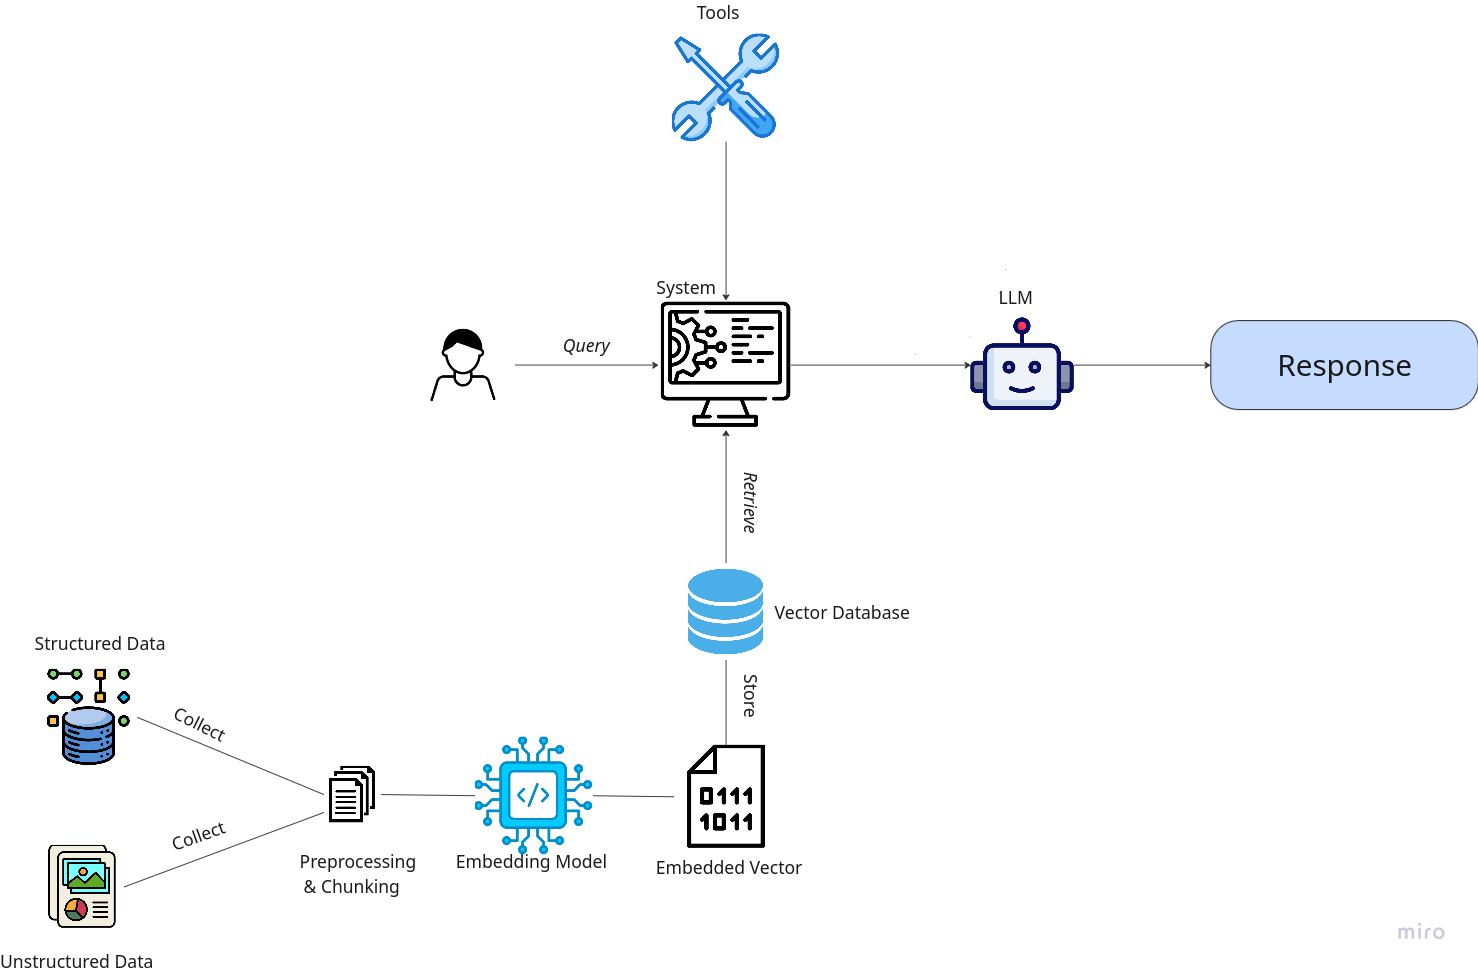
\includegraphics[width=\linewidth]{rag_pipeline.png}
    \caption{A RAG pipeline}
    \label{fig:placeholder}
\end{figure}

  \subsection{The Role of External Knowledge}
In the context of information-intensive tasks, relying solely on the pre-trained knowledge of LLMs presents significant challenges. The integration of external knowledge sources serves three critical functions within the RAG framework:

\begin{enumerate}
    \item \textbf{Mitigating Knowledge Cutoffs (Temporal Agility):} 
    LLMs are trained on static datasets collected up to a specific point in time. Consequently, they are \textit{blind} to events or data generated post-training. In the movie domain, where new films are released weekly and ratings fluctuate in real-time, this limitation is critical. External knowledge bases allow the system to access the most current information without the prohibitive computational cost of continuous model retraining (Fine-tuning).

    \item \textbf{Domain Specificity and Granularity:} 
    While foundation models possess broad general knowledge, they often lack depth in specialized domains. An external database ensures the model has access to precise, granular metadata—such as specific production budgets, obscure cast members of indie films, or exact revenue figures—that may be underrepresented or "forgotten" in the model's vast parametric memory.

    \item \textbf{Explainability and Trust:} 
    When an LLM generates an answer purely from its weights, the information source is opaque (a "black box"), making it impossible to verify. By explicitly retrieving documents or graph nodes, RAG enables "source tracking." The system can provide citations (e.g., \textit{"According to the TMDB record for 'Inception'..."}), thereby allowing users to verify the accuracy of the recommendations and reducing the risk of confident hallucinations.
\end{enumerate}
\section{Vector-Based Retrieval (Dense Retrieval)}
\label{sec:vector_retrieval}
    \subsection{Semantic Embeddings}
    % Giải thích Sentence-BERT: Biến câu "Iron Man" thành vector [0.1, 0.5, ...].
    In a Retrieval-Augmented Generation system, the retrieval engine must bridge the gap between natural language queries and stored documents. Traditional keyword-based methods (e.g., TF-IDF \cite{tfidf}) rely on exact lexical overlapping, which fails to capture synonyms or contextual meaning. To overcome this, we employ Dense Semantic Embeddings.

\subsubsection{Concept}
Semantic embedding is the process of transforming text input (words, sentences, or paragraphs) into a fixed-size vector of real numbers in a high-dimensional space. Formally, given an embedding function $f_\theta$ and a text sequence $S$, the output is a vector $v$:
\begin{equation}
    v = f_\theta(S) \in \mathbb{R}^d
\end{equation}
where $d$ is the dimensionality of the vector space (typically 384, 768, or 1536 depending on the model).



In this latent space, the geometric distance between two vectors corresponds to their semantic similarity. For instance, in the movie domain, the vector for \textit{"Interstellar"} will be closer to \textit{"Space exploration"} than to \textit{"Romantic comedy"}, even if the words "space" or "exploration" do not appear explicitly in the movie's title.

\subsubsection{Sentence-BERT (SBERT)}
While models like BERT \cite{devlin-etal-2019-bert} revolutionized NLP, they are computationally expensive for retrieval tasks because they require feeding both sentences into the network simultaneously (Cross-Encoder). 

The Sentence-BERT (SBERT) \cite{sbert}, a modification of the BERT network that uses \textbf{Siamese Networks} to derive semantically meaningful sentence embeddings. SBERT processes sentences independently to generate fixed vectors, allowing for highly efficient comparison using Cosine Similarity. This architecture enables the pre-computation (indexing) of millions of movie descriptions, making real-time retrieval feasible.

\subsubsection{Gemini Embedding models \cite{geminiembeddings}}
Semantic embedding is the process of transforming text input (words, sentences, or paragraphs) into a fixed-size vector of real numbers in a high-dimensional space. Formally, given the Gemini embedding function $E_{Gemini}$ and a text sequence $S$, the output is a dense vector $v$:
\begin{equation}
    v = E_{Gemini}(S) \in \mathbb{R}^d
\end{equation}
where $d$ represents the dimensionality of the vector space (typically $d=768$ for standard Gemini embedding models). 

In this latent space, the geometric distance between two vectors corresponds to their semantic similarity. For instance, the vector for \textit{"The Dark Knight"} will be spatially closer to \textit{"Crime thriller"} than to \textit{"Romantic comedy"}, enabling the system to understand content beyond mere keyword matching.

\subsubsection{Gemini Embedding Architecture}
Unlike traditional open-source models (e.g., Word2Vec \cite{w2v}) which generate static embeddings, Gemini utilizes a modern Transformer-based architecture \cite{attention} optimized for semantic retrieval tasks. Key advantages utilized in this project include:

\begin{itemize}
    \item \textbf{Task-Specific Embeddings:} The Gemini API distinguishes between \textit{retrieval\_query} (the user's question) and \textit{retrieval\_document} (the knowledge base content). This asymmetry allows the model to optimize the vector space specifically for matching questions to answers, rather than just matching similar sentences.
    \item \textbf{Multilingual Support:} Trained on a massive, diverse corpus, Gemini embeddings demonstrate superior performance in capturing nuances across different languages, which is crucial for handling movie titles and descriptions that may contain international context.
    \item \textbf{High Dimensionality:} With a vector dimension of 768, the model captures a richer set of semantic features compared to smaller models (e.g., 384 dimensions), resulting in higher precision during the retrieval phase.
\end{itemize}
    \subsection{Similarity Measures}
    Information retrieval relies on measuring the distance between the query vector $q$ and document vector $d$. The most common metric is Cosine Similarity:
    \begin{equation}
        \text{CosSim}(q, d) = \frac{q \cdot d}{\|q\| \|d\|} = \frac{\sum_{i=1}^{n} q_i d_i}{\sqrt{\sum_{i=1}^{n} q_i^2} \sqrt{\sum_{i=1}^{n} d_i^2}}
    \end{equation}

    \subsection{Approximate Nearest Neighbor (ANN) Search}
 In a real-world scenario with a large corpus of movie data, calculating the Cosine Similarity between the query vector and \textit{every} stored vector (Exact k-NN) is computationally prohibitive. This "brute-force" approach has a time complexity of $O(N \cdot d)$, where $N$ is the number of documents and $d$ is the vector dimension. To ensure low-latency retrieval, this system employs Approximate Nearest Neighbor (ANN) algorithms.



\subsubsection{The Trade-off: Precision vs. Speed}
ANN algorithms relax the guarantee of finding the absolute "closest" neighbor in exchange for a significant reduction in search time (typically achieving logarithmic complexity $O(\log N)$). The system organizes vectors into an index structure that allows the retrieval engine to traverse the vector space efficiently, inspecting only a small subset of candidate vectors that are likely to be relevant.

\subsubsection{Hierarchical Navigable Small World (HNSW)}
For this project, we utilize the HNSW algorithm \cite{malkov2018efficient}, which is currently the state-of-the-art method for vector indexing (used by default in vector databases like Qdrant and Neo4j).

HNSW constructs a multi-layered graph structure:
\begin{itemize}
    \item[] \textbf{Upper Layers (Express Lanes):} Contain sparse connections (long-range links) allowing the search algorithm to quickly "zoom in" on the general neighborhood of the query vector.
    \item[] \textbf{Lower Layers (Local Roads):} Contain dense connections for fine-grained traversal to identify the specific nearest neighbors.
\end{itemize}

This hierarchical structure mimics the "six degrees of separation" phenomenon, allowing the system to locate the most relevant movie vectors among thousands of entries in milliseconds.
    
    \subsection{Limitations in Multi-hop Reasoning}

While vector-based retrieval excels at finding semantically similar documents, it encounters a fundamental bottleneck when handling Multi-hop Queries—questions that require retrieving information from multiple distinct documents and chaining them together logically.

\subsubsection{The \textit{Information Flattening} Problem}
Vector embedding models compress complex structured data (entities and relationships) into a single flat vector in a latent space. In this process, the explicit structural dependencies between entities are often lost or flattened.
\begin{itemize}
    \item \textbf{Vector Proximity $\neq$ Logical Relationship:} Two vectors might be close in space because they share similar keywords (e.g., "Hollywood", "Cinema"), not because there is a verified factual link between them.
    \item \textbf{Loss of Transitivity:} If Fact A is in Document 1 and Fact B is in Document 2, a vector search engine treats them as independent. It lacks the mechanism to perform transitive reasoning (i.e., if $A \rightarrow B$ and $B \rightarrow C$, then $A \rightarrow C$).
\end{itemize}



\subsubsection{Case Study: The "Tom Cruise" Example}
Consider the complex query: \textit{"Who is the ex-wife of Tom Cruise that starred in a horror movie?"}

\begin{enumerate}
    \item \textbf{Vector Search Failure:} A vector-based system will embed this query and look for documents containing terms like "Tom Cruise", "Ex-wife", and "Horror".
    \begin{itemize}
        \item \textit{Likely Outcome:} It might retrieve a biography of Tom Cruise (mentioning his wives) OR a list of horror movies. It often fails to connect the specific wife (Nicole Kidman) to the specific genre (Horror) if those facts reside in separate documents. It might erroneously return "Interview with the Vampire" (because it features Tom Cruise and is a horror movie).
    \end{itemize}
    
    \item \textbf{The Structural Gap:} To answer correctly, the system must traverse a specific logical path:
    $$ \text{Tom Cruise} \xrightarrow{\text{SPOUSE}} \text{Nicole Kidman} \xrightarrow{\text{ACTED\_IN}} \text{The Others} \xrightarrow{\text{GENRE}} \text{Horror} $$
    Vector search has no concept of these edges (arrows) and thus struggles to "hop" from Cruise to Kidman and then to her movies \cite{xiong2020answering}.
\end{enumerate}

This limitation necessitates a shift towards \textbf{Graph-based RAG}, where these relationships are explicitly modeled as edges that can be traversed.

% --- SECTION 2.4: KNOWLEDGE GRAPHS ---
\section{A General Framework for Graph Retrieval-Augmented Generation}
\begin{figure}
    \centering
    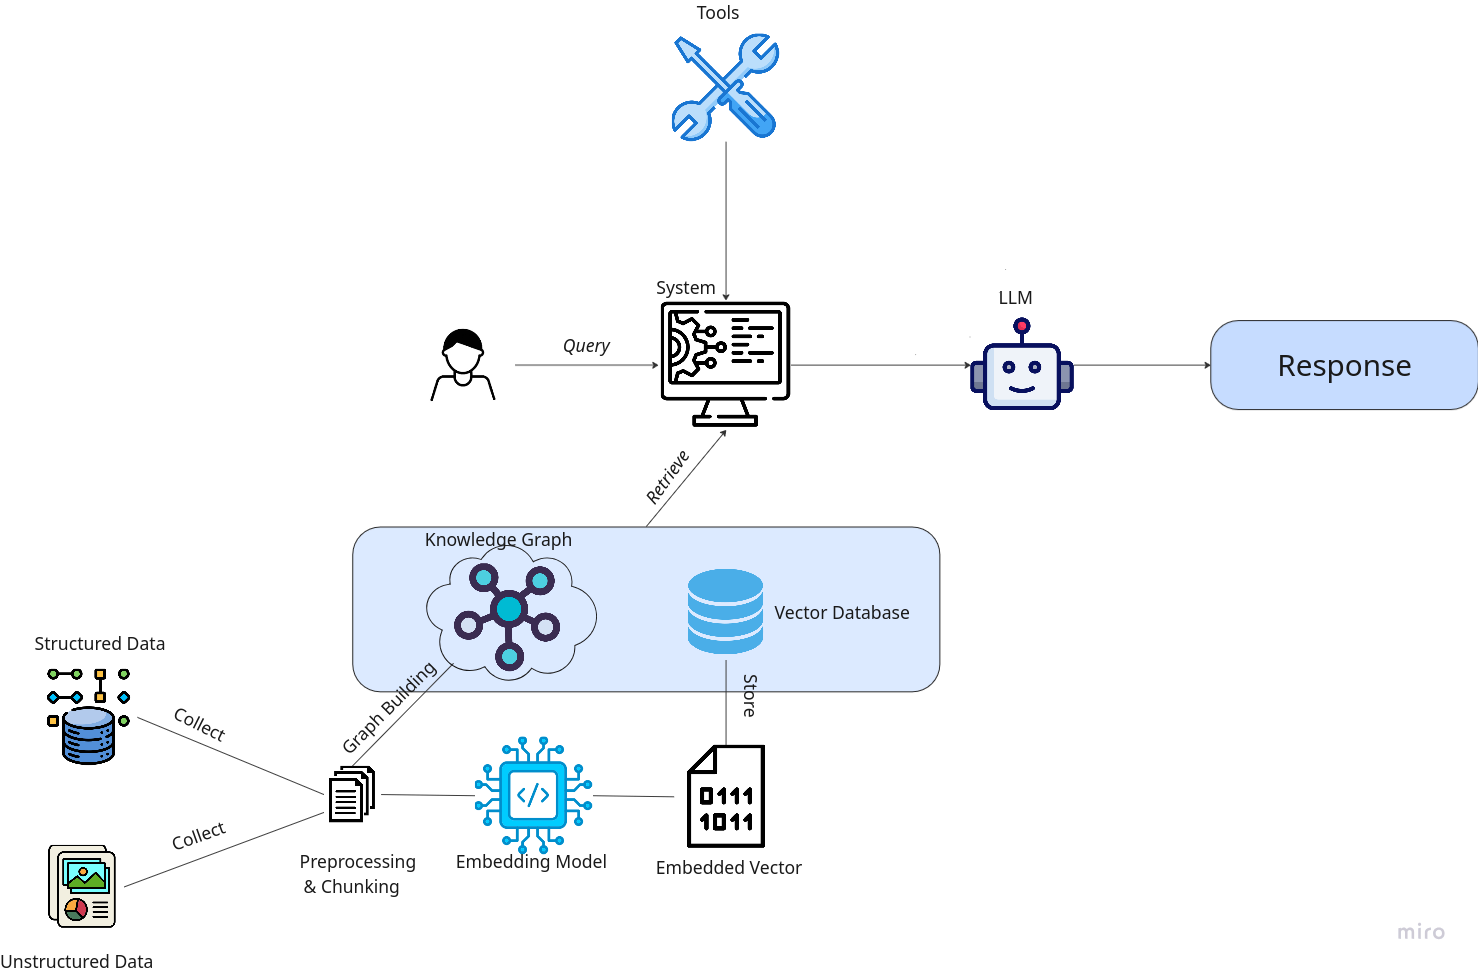
\includegraphics[width=\linewidth]{graphrag.png}
    \caption{A Simple GraphRAG Pipeline}
    \label{fig:GraphRAG}
\end{figure}
\subsection{Overview and Problem Formulation}
Traditional Retrieval-Augmented Generation (RAG) systems primarily rely on vector similarity to retrieve flat text chunks \cite{lewis2020rag}. While effective for surface-level queries, this approach often fails to capture the intricate relational dependencies essential for complex reasoning. To address this limitation, we propose a holistic framework for GraphRAG that explicitly models information as a structured network. Formally, given a user query $Q$ and a graph-structured knowledge source $G$, the system operates through a sophisticated pipeline of five interconnected components: the Query Processor ($\Omega_{Processor}$), the Retriever ($\Omega_{Retriever}$), the Organizer ($\Omega_{Organizer}$), the Generator ($\Omega_{Generator}$), and the underlying Graph Data Source ($G$).



The inference process is not merely a retrieval task but a sequential transformation of information. It begins with the projection of the natural language query into a graph-compatible representation, followed by the topological exploration of the graph, the refinement of the extracted subgraph, and finally, the generative synthesis of the answer. Mathematically, this end-to-end workflow can be formalized as:
\begin{equation}
    A = \Omega_{Generator}\Big(\Omega_{Organizer}\big(\Omega_{Retriever}(\hat{Q}, G), \hat{Q}\big), Q\Big)
\end{equation}
where $\hat{Q}$ denotes the processed query and $A$ represents the final generated answer.


\subsection{The Query Processor: Bridging the Modality Gap}
The first challenge in GraphRAG \cite{han2025retrievalaugmentedgenerationgraphsgraphrag} is bridging the modality gap between the unstructured natural language of the user ($Q$) and the structured schema of the graph ($G$). The Query Processor ($\Omega_{Processor}$) serves as this bridge. Unlike standard RAG which simply embeds the query, GraphRAG requires a semantic decomposition of the input.

This process begins with \textbf{Named Entity Recognition (NER) and Linking}. The system must identify specific mentions within the query and map them to unique nodes $v \in V$ within the graph. However, simple string matching is insufficient due to ambiguity. For instance, the token "Matrix" could refer to a mathematical concept or a movie franchise. Therefore, we employ a context-aware entity linking mechanism that utilizes the surrounding textual context to resolve these ambiguities, ensuring that the identified "Anchor Nodes" are semantically accurate.

Following entity identification, the processor performs \textbf{Relational Extraction}. This step is crucial for guiding the traversal direction. By analyzing the query's predicate (e.g., "directed by" or "sequel to"), the system identifies the specific edge types $e \in E$ that are relevant, thereby pruning the search space before retrieval even begins. Furthermore, for complex, multi-hop questions such as "What other movies did the director of Interstellar make?", the processor employs Query Decomposition\cite{touvron2023llama}. The query is broken down into a logical chain of sub-queries $\{q_1, q_2, \dots, q_k\}$, where the output of one retrieval step serves as the input anchor for the next, mirroring the human cognitive process of step-by-step reasoning.

\subsection{The Retriever: Topological Exploration}
Once the query is processed into a structured format $\hat{Q}$, the Retriever ($\Omega_{Retriever}$) executes the core lookup operation. Unlike the "Text-in, Text-out" paradigm of traditional retrievers, GraphRAG employs a "Text-in, Graph-out" approach, extracting a relevant subgraph $G_{sub} \subset G$ .

We employ a hybrid retrieval strategy that combines the precision of heuristics with the semantic breadth of representation learning. On one hand, \textbf{Heuristic Retrieval} utilizes algorithms such as Breadth-First Search (BFS) to explore the $k$-hop neighborhood of the anchor nodes. This ensures that directly connected entities—which often contain the most pertinent information—are captured. However, heuristic methods are limited by the explicit connections in the graph.

To overcome this, we integrate \textbf{Learning-based Retrieval} using Graph Neural Networks (GNNs). GNNs allow the system to capture implicit structural roles and high-order proximity \cite{wu2023comprehensive}. Through a message-passing mechanism, a node aggregates features from its neighbors, refining its own representation \cite{scarselli2008gnn, kipf2017gcn}:
\begin{equation}
    h_v^{(l)} = \sigma \left( \sum_{u \in \mathcal{N}(v)} W^{(l)} \cdot \text{AGG}\left(h_u^{(l-1)}, h_v^{(l-1)}\right) \right)
\end{equation}
This allows the retriever to identify nodes that are semantically relevant to the query embedding even if they are not immediate neighbors, thus enhancing the recall of the system.



\subsection{The Organizer: Context Refinement and Linearization}
A raw retrieved subgraph is often noisy and too complex for direct consumption by a Large Language Model (LLM). The Organizer ($\Omega_{Organizer}$) acts as a filter and translator. Its primary function is to optimize the context $\hat{C}$ to maximize the generator's performance while minimizing token usage.

The first step in this phase is \textbf{Graph Pruning}. Due to the "small-world" nature of many graphs, a 2-hop expansion can result in thousands of nodes, leading to "Graph Explosion." The organizer applies a relevance scoring function—typically based on the cosine similarity between the node embeddings and the query vector—to prune irrelevant branches. Only the paths that contribute significantly to the reasoning chain are retained.

Subsequently, the refined subgraph must be converted into a linear sequence, a process known as \textbf{Verbalization}. Since LLMs process sequential text, the organizer linearizes the graph structure. We adopt a "Reasoning Path" linearization strategy, where connected triples are merged into coherent natural language sentences (e.g., "Node A is connected to Node B via Relation R") rather than a disjointed list of tuples. This narrative format preserves the logical flow of information, making it easier for the LLM to follow the chain of evidence \cite{attention}.

\subsection{The Generator: Synthesis and Provenance}
The final component, the Generator ($\Omega_{Generator}$), synthesizes the answer. In our framework, we leverage the generative capabilities of modern LLMs, enhanced by \textbf{Graph-Grounded Prompting}. The linearized graph context is injected into the prompt with specific instructions to perform "closed-book" reasoning—meaning the model must rely solely on the provided graph data. Crucially, the generator is configured to provide \textbf{provenance} for its assertions. By citing the specific edges or nodes used to derive an answer, the system significantly mitigates the hallucination problem common in generative AI, ensuring that every claim is traceable back to the source Knowledge Graph.
\section{Knowledge Graph: Foundations and Mechanisms in GraphRAG}
\begin{figure}
    \centering
    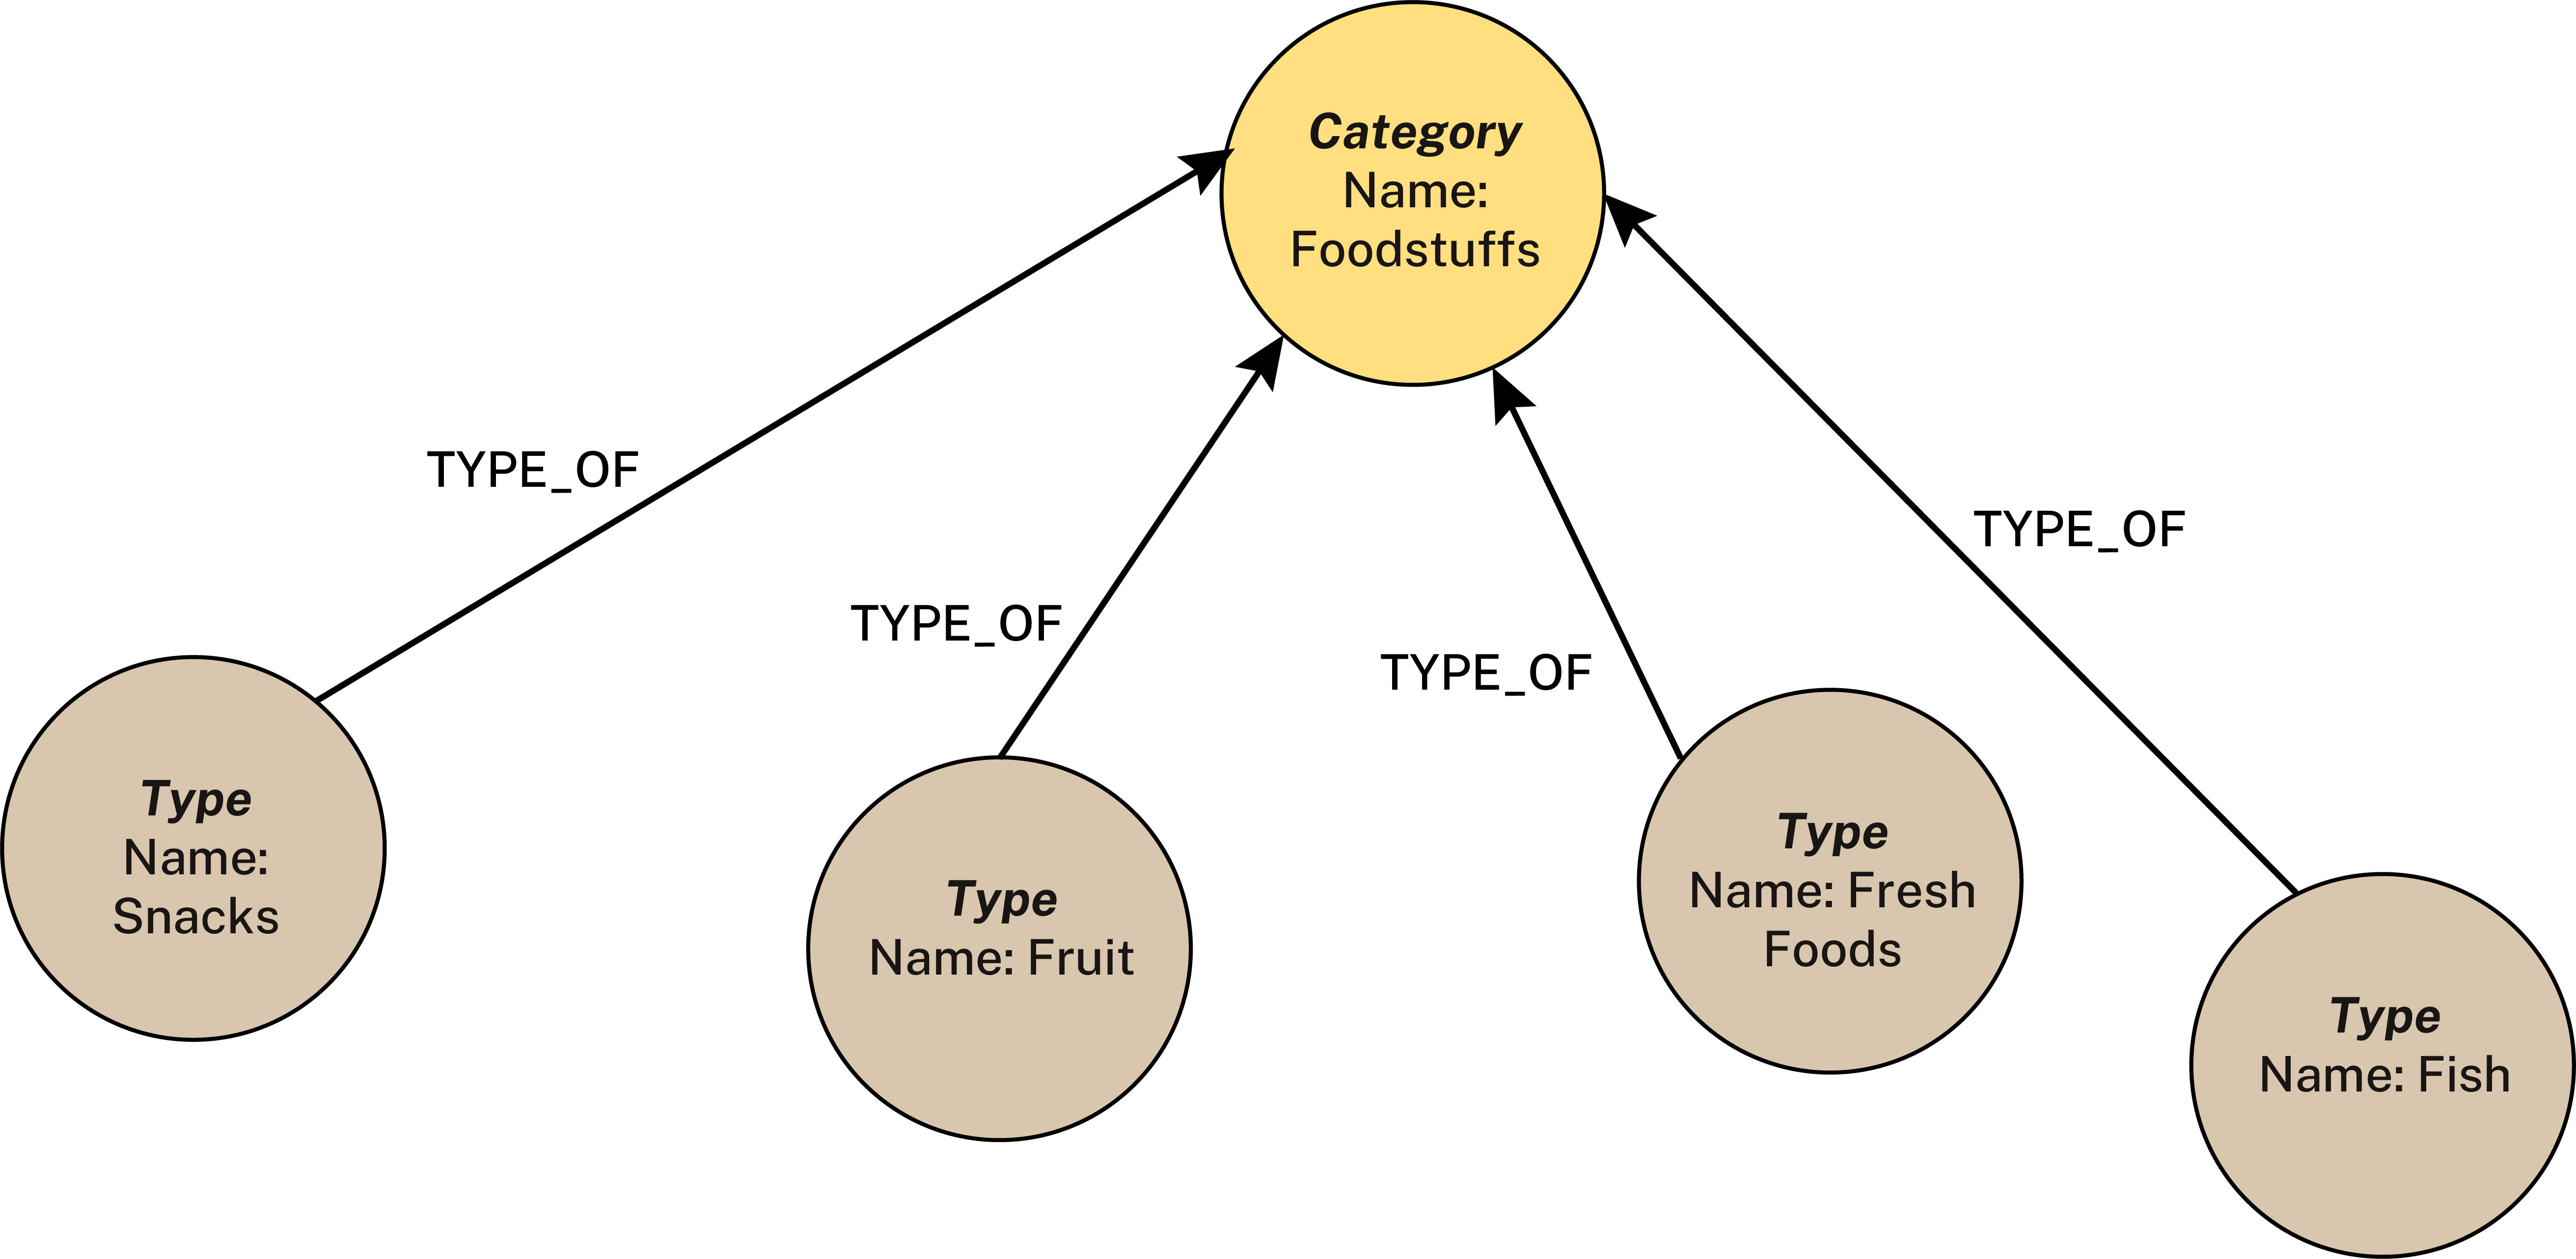
\includegraphics[width=\linewidth]{kg.png}
    \caption{Example Knowledge Graph}
    \label{fig:graph}
\end{figure}

In the context of Graph Retrieval-Augmented Generation (GraphRAG), the Knowledge Graph (KG) serves as the structured cognitive backbone. Unlike unstructured vector databases, a KG explicitly models information as a network of entities connected by well-defined relationships. It can encompass general knowledge or specialized domains. The diverse topology of a KG, comprising entities, edges, paths, and subgraphs, provides a robust substrate for enhancing downstream tasks such as Question Answering (QA), Fact-Checking, and Complex Reasoning.

This section provides a comprehensive review of the lifecycle of Knowledge Graphs within the RAG framework, ranging from their construction to the intricate mechanisms of retrieval and generation.

\subsection{Application Scenarios}
The utility of KGs in RAG spans multiple high-stakes domains \cite{graphrag2025}:
\begin{itemize}
    \item \textbf{Question Answering (QA):} For queries like \textit{"Were there fossil fuels when humans evolved?"}, the answer is rarely contained in a single document span. GraphRAG leverages KGs to traverse relationships across disparate documents, providing necessary context and multi-hop reasoning capabilities that standard LLMs lack.
    \item \textbf{Fact-Checking:} Verification requires cross-referencing claims against reliable sources. By mapping a statement onto the KG, the system can identify discrepancies or confirmations within the relational structure, offering an evidence-based validation process.
    \item \textbf{Knowledge Graph Completion:} Beyond simple retrieval, GraphRAG can be employed to predict missing links (triplets), thereby enhancing the comprehensiveness of the graph itself through inductive reasoning.
    \item \textbf{Cybersecurity \& Defense:} In security analysis, KGs model complex attack patterns and vulnerabilities. GraphRAG provides insights into potential threat vectors by tracing the paths between system components and known exploit signatures.
\end{itemize}

\subsection{Knowledge Graph Construction Methodologies}
The efficacy of a GraphRAG system is strictly upper-bounded by the quality of its underlying graph. Construction methodologies have evolved from manual curation to automated, LLM-driven pipelines.

\subsubsection{Manual and Rule-Based Construction}
Early KGs relied on crowd-sourced human annotation or strict ontological rules.
\begin{itemize}
    \item[] \textit{Manual:} Highly accurate but labor-intensive and difficult to scale.
    \item[] \textit{Rule-based:} Systems utilize custom parsers. Recent approaches employ traditional NLP pipelines (e.g., SpaCy for Entity Recognition) to parse raw text into structured assertions.
\end{itemize}

\subsubsection{LLM-Based Construction}
Addressing the scalability bottleneck, recent research focuses on using Large Language Models (LLMs) to automatically distill KGs from unstructured corpora \cite{graphrag2025}.
\begin{itemize}
    \item[] \textbf{Schema-Free Extraction:} Methods treat text passages as nodes and determine connections based on semantic similarity encoding.
    \item[] \textbf{Chunk-and-Extract:} The GraphRAG approach involves dividing documents into chunks, prompting an LLM to extract all entities (names, types, descriptions) and their relationships. A second pass summarizes these elements to resolve coreferences, effectively creating a KG that represents the document set without a ground-truth ontology.
    \item[] \textbf{Clustering:} Tools combine LLM embeddings with clustering algorithms to group semantically similar concepts into unified nodes.
\end{itemize}


\subsection{Retrieval Mechanisms on Knowledge Graphs}
Retrieval on KGs is fundamentally different from vector search. It is a two-stage process involving \textit{Seed Identification} followed by \textit{Structure Expansion}.

\subsubsection{Stage 1: Identifying Seed Entities ($V_{seed}$)}
Before traversing the graph, the system must anchor the user query to specific nodes.
\begin{itemize}
    \item[] \textbf{Direct Extraction:} Traditional NER tools extract named entities from the query.
    \item[] \textbf{Hypothesis Generation:} Methods use an LLM to generate a hypothetical answer, then extract entities from both the query and the hypothesis to increase recall.
    \item[] \textbf{Similarity Search:} To handle ambiguity, systems compute vector similarity between the query embedding and node embeddings, selecting the top-$k$ most similar nodes as seeds.
\end{itemize}

\subsubsection{Stage 2: Core Retrieval Strategies}
Once seeds are identified, the system mines the graph for context. We categorize the retrieval algorithms as follows:

\textbf{A. Traversal-Based Retriever:}
These methods explicitly "walk" the graph edges.
\begin{itemize}
    \item[] \textit{Path Extraction:} Algorithms extract all paths of length $L \le 2$ connecting seed entities. Reasoning on Knowledge utilizes \textbf{Personalized PageRank (PPR)} to identify the most influential paths relative to the query.
    \item[] \textit{Beam Search:} Approaches employ beam search to explore the graph iteratively, expanding only the most promising nodes at each step based on a relevance scoring model.
    \item[] \textit{Pruning:} To avoid graph explosion, methods predict the expected hop count ($h_Q$) and use an LLM to dynamically prune irrelevant branches during traversal.
\end{itemize}

\textbf{B. Subgraph-Based Retriever:}
Instead of individual paths, these methods retrieve the entire ego-network (1-hop or 2-hop neighborhood) surrounding the seeds.
\begin{itemize}
    \item[] The retrieved subgraphs are often unioned together. Recent works propose partitioning large subgraphs into smaller clusters and ranking them, feeding only the top-ranked clusters to the generator.
\end{itemize}

\textbf{C. GNN-Based Retriever:}
Graph Neural Networks (GNNs) are used to capture complex structural signals \cite{scarselli2008gnn}.
\begin{itemize}
    \item[] \textit{GNN-RAG} trains a GNN for node classification, where the target is to predict the answer node. During inference, the shortest path to the highest-probability node is retrieved.
    \item[] \textit{Conditional GNNs:} Methods initialize only the seed nodes with non-zero representations and propagate features. An attention mechanism prunes edges at each layer, effectively learning a "reasoning path" in a differentiable manner.
\end{itemize}

\textbf{D. Agentic and Rule-Based Retriever:}
\begin{itemize}
    \item[] \textit{Agent-based:} Systems treat retrieval as a tool-use problem. They generate executable code (Python/SQL/SPARQL) to search the KG, allowing for complex aggregation and filtering operations that simple traversal cannot handle.
    \item[] \textit{Template-based:} Methods decompose queries into sub-queries and match them against pre-defined logical chain templates to retrieve specific path patterns.
\end{itemize}


\subsection{The Organizer: Refining Structured Knowledge}
Raw retrieved data (triples/subgraphs) is often not in an optimal format for LLM consumption. The Organizer component bridges this gap.

\subsubsection{Verbalization (Graph-to-Text)}
\begin{itemize}
    \item[] \textbf{Tuple-Based:} The simplest approach lists facts as triples `(Entity1, Relation, Entity2)`. This is token-efficient but lacks semantic nuance.
    \item[] \textbf{Template-Based:} Converting triples into natural language sentences using templates (e.g., "The [Relation] of [Entity1] is [Entity2]").
    \item[] \textbf{Model-Based:} Advanced methods use a "Knowledge Rewriter"—a fine-tuned LLM—to summarize the retrieved subgraph into a coherent paragraph, preserving the logic while reducing token count.
\end{itemize}

\subsubsection{Reranking}
To mitigate the LLM's "lost-in-the-middle" phenomenon, retrieved facts must be ordered by relevance.
\begin{itemize}
    \item[] \textit{Cross-Encoders:} Methods employ Cross-Encoders or LLM-based scoring to re-rank triples.
    \item[] \textit{Temporal Ordering:} For Temporal KGs, paths are ordered chronologically, prioritizing recent information.
\end{itemize}

\subsection{The Generator: Synthesis Architectures}
The final answer generation leverages the processed graph data.
\begin{itemize}
    \item[] \textbf{LLM-Based:} The dominant approach injects the verbalized graph into the system prompt of models like Gemini or LLaMA \cite{team2023gemini, touvron2023llama}. Techniques like \textit{LoRA} fine-tuning are often used to adapt the model to the specific graph schema.
    \item[] \textbf{GNN-Based:} For discrimination tasks (e.g., predicting an entity category), the system fuses the text embedding of the query with the graph embedding of candidate nodes to predict the outcome probability directly, bypassing textual generation.
\end{itemize}

\subsection{Resources and Tools}
The ecosystem for GraphRAG is supported by robust data resources and frameworks.
\begin{itemize}
    \item[] \textbf{Data Sources:} Freebase (general facts), ConceptNet (semantic common sense), and Wikidata (structured encyclopedia).
    \item[] \textbf{Tooling:} LangChain provides abstractions for chaining graph retrieval steps \cite{langchain2023}, while Microsoft's GraphRAG offers a complete implementation of the text-to-graph pipeline.
\end{itemize}

\chapter{Methodology and System Implementation}

This section details the concrete implementation of the GraphRAG-powered conversational agent. We translate the holistic framework proposed in Section II into a functional architecture. The system is designed as a neuro-symbolic pipeline, integrating the probabilistic reasoning of Google's Gemini models with the deterministic structure of a Graph Database.

This chapter details the architectural design and implementation of the proposed Graph Retrieval-Augmented Generation (GraphRAG) system. We present a comprehensive pipeline that integrates a neuro-symbolic approach, combining the semantic understanding of Large Language Models (LLMs) with the structured reasoning capabilities of Knowledge Graphs.

\section{System Architecture Overview}
\label{sec:system_architecture}

The proposed system is architected as a modular pipeline consisting of five interconnected components, designed to transform a raw user query into a factually grounded response.


The workflow operates sequentially as follows:
\begin{enumerate}
    \item \textbf{Query Processor:} The entry point that parses, decomposes, and enriches the user's natural language input.
    \item \textbf{Retrieval Module:} A hybrid engine that executes parallel searches on both the Vector Database (Qdrant) and the Graph Database (Neo4j).
    \item \textbf{Context Organizer:} A post-processing unit that reranks, prunes, and structures the retrieved information to optimize the LLM's context window.
    \item \textbf{Knowledge Storage:} The dual-memory system comprising unstructured vector embeddings and structured graph relationships.
    \item \textbf{LLM Generator:} The generative component (Google Gemini 2.5 Flash) that synthesizes the final answer based on strict grounding rules.
\end{enumerate}


\section{Data Acquisition and Graph Construction}
\label{sec:data_construction}

\subsection{Dataset Curation}
We utilize the \textbf{TMDB (The Movie Database)} API as the primary data source. The curated dataset comprises over \textbf{1,000 movies} spanning from the 1970s to 2024. This subset focuses on high-popularity films across diverse genres to ensure a dense network of relationships suitable for testing multi-hop reasoning capabilities. Key attributes collected include titles, cast members (top 8 billing), directors, genres, plot overviews, and user ratings.
\subsection{Data Preprocessing and Cleansing}
\label{sec:data_preprocessing}

Raw data retrieved from the TMDB API typically contains noise, missing values, and inconsistencies that can degrade the performance of both vector retrieval and graph traversal. To ensure high data quality, we implemented a rigorous preprocessing pipeline comprising four key stages:

\subsubsection{Filtering and Selection}
To align with the project's scope of recommendation for general audiences, we applied strict filtering criteria:
\begin{itemize}
    \item[] \textbf{Temporal Window:} We restricted the dataset to movies released between the 1970s and 2024 to focus on modern cinema while retaining classic context.
    \item[] \textbf{Popularity Threshold:} Only movies with a meaningful vote count (typically $>50$ votes) were retained to eliminate obscure entries with sparse metadata.
    \item[] \textbf{Cast Pruning:} To prevent "supernode" explosion in the graph (where a single generic extra connects thousands of unrelated movies), we limited the \texttt{(:Actor)} nodes to the \textbf{top-8 billed cast members} per movie. This focuses the graph on the primary contributors to the film's identity.
\end{itemize}

\subsubsection{Text Normalization}
The textual attributes, particularly the movie `overview` (plot summary) and `title`, serve as the input for vector embeddings. These fields underwent the following normalization steps:
\begin{itemize}
    \item \textbf{Cleaning:} Removal of HTML tags, extra whitespace, and non-standard ASCII characters.
    \item \textbf{Case Folding:} While modern embedding models are case-sensitive, we normalized specific metadata fields (like genres and keywords) to lowercase to ensure consistent Cypher matching (e.g., treating "Sci-Fi" and "sci-fi" as identical).
\end{itemize}

\subsubsection{Entity Disambiguation}
A critical challenge in graph construction is entity identity. A string match for "Chris Evans" could refer to the famous actor or a different crew member. To resolve this:
\begin{itemize}
    \item[] We utilized the unique \texttt{tmdb\_id} as the primary key for all \texttt{(:Person)} and \texttt{(:Movie)} nodes, rather than their string names.
    \item[] Duplicate entities were merged. If an actor appeared in multiple movies, a single \texttt{(:Person)} node was created/updated, ensuring the graph connectivity is based on unique identities.
\end{itemize}

\subsubsection{Missing Data Handling}
Incomplete records were handled based on the criticality of the missing field:
\begin{itemize}
    \item[] Records missing a \texttt{title} or \texttt{overview} were discarded, as they cannot be effectively embedded.
    \item[] Records missing specific relationships (e.g., no director listed) were retained but flagged, allowing the graph to remain functional even with partial topology.
\end{itemize}

\begin{table}[h]
\centering
\caption{Summary of Data Preprocessing Statistics}
\label{tab:preprocessing_stats}
\begin{tabular}{|l|l|l|}
\hline
\textbf{Metric} & \textbf{Raw Data} & \textbf{Processed Data} \\ \hline
Total Movies & $\sim$ 2,000 & 1,523 \\ \hline
Actors per Movie & Full Cast ($\sim$30+) & Top 8 (Truncated) \\ \hline
Time Range & 1900 - 2024 & 1970 - 2024 \\ \hline
Format & Nested JSON & Normalized Graph Entities \\ \hline
\end{tabular}
\end{table}
\subsection{Graph Schema Design}
To effectively model the cinematic domain, we constructed a Knowledge Graph defined by the following schema:


\begin{itemize}
    \item \textbf{Nodes (Entities):}
    \begin{itemize}
        \item \texttt{(:Movie)}: The central entity containing metadata and embeddings.
        \item \texttt{(:Person)}: Further specialized into \texttt{(:Director)} and \texttt{(:Actor)}.
        \item \texttt{(:Genre)}: Categorical nodes (e.g., Action, Sci-Fi).
        \item ...
    \end{itemize}
    
    \item \textbf{Relationships (Edges):}
    \begin{itemize}
        \item \texttt{(:Actor)-[:ACTED\_IN]->(:Movie)}: Captures casting information.
        \item \texttt{(:Director)-[:DIRECTED]->(:Movie)}: Captures directorial authorship.
        \item \texttt{(:Movie)-[:HAS\_GENRE]->(:Genre)}: Maps films to categories.
        \item \texttt{(:Movie)-[:SIMILAR\_TO]->(:Movie)}: Represents content-based similarity derived from plot embeddings.
        \item ...
    \end{itemize}
\end{itemize}

\section{Query Processing Module}
\label{sec:query_processing}

Unlike "naive" RAG systems that directly embed the raw query, our system employs an enhanced Query Processor to bridge the gap between natural language and graph topology.

\subsection{Entity and Relation Extraction}
We leverage an LLM-based extraction step to identify key entities and semantic intents within the query:
\begin{itemize}
    \item \textbf{Named Entity Recognition (NER):} Identifies specific instances of \textit{Person} (e.g., "Christopher Nolan"), \textit{Movie} titles, and \textit{Temporal} markers (e.g., "2010s").
    \item \textbf{Relation Extraction:} Maps user intent to graph edges. For example, "worked with" implies a pattern of \texttt{(:Person)-[:ACTED\_IN]->(:Movie)<-[:ACTED\_IN]-(:Person)}.
\end{itemize}

\subsection{Decomposition and Expansion}
To handle complex queries, the processor applies:
\begin{enumerate}
    \item \textbf{Query Decomposition:} Multi-hop queries are broken down into logical sub-queries. For instance, the query \textit{"Which actors worked with Nolan and also in Inception?"} is split into:
    \begin{itemize}
        \item $Q_1$: Find actors linked to "Christopher Nolan" via \texttt{[:DIRECTED]}.
        \item $Q_2$: Find actors linked to "Inception" via \texttt{[:ACTED\_IN]}.
        \item Operation: Intersection ($Q_1 \cap Q_2$).
    \end{itemize}
    \item \textbf{Query Expansion:} Synonyms are generated to increase recall (e.g., "thriller" $\rightarrow$ ["suspense", "mystery"]).
    \item \textbf{Confidence Scoring:} Each processed query is assigned a confidence score based on ambiguity levels to guide the retrieval strategy.
\end{enumerate}

\section{Hybrid Retrieval Strategy}
\label{sec:retrieval_strategy}

The core of our methodology is a two-stage hybrid retrieval process that enriches vector search results with graph traversal.

\subsection{Stage 1: Vector Retrieval}
The system first performs a dense retrieval using \textbf{Qdrant}.
\begin{itemize}
    \item \textbf{Embedding Model:} \texttt{text-embedding-004} (Google).
    \item \textbf{Metric:} Cosine Similarity.
    \item \textbf{Configuration:} We retrieve the Top-$K$ ($K=8$) movies with a similarity threshold of $0.5$.
\end{itemize}

\subsection{Stage 2: Graph Enrichment}
Using the retrieved movies as "anchor nodes," the system performs a traversal in \textbf{Neo4j} to fetch contextual neighborhoods:
\begin{enumerate}
    \item \textbf{1-Hop Expansion:} Retrieving immediate connections (Director, Cast, Genre) to provide factual metadata.
    \item \textbf{2-Hop Traversal:} Identifying "sibling" nodes (e.g., other movies by the same director) to support recommendation tasks.
\end{enumerate}

Formally, the Cypher query structure for enrichment is defined as:
\begin{verbatim}
MATCH (m:Movie)-[r:ACTED_IN|DIRECTED|HAS_GENRE]-(related)
WHERE m.title IN $retrieved_movies
RETURN m, r, related
\end{verbatim}

\section{Context Organization and Generation}
\label{sec:context_generation}

\subsection{Context Refinement}
Raw retrieved data is often redundant or noisy. The \textbf{Context Organizer} applies a three-step filtering process:
\begin{enumerate}
    \item \textbf{Diversity Pruning:} To avoid repetitive information, we calculate the cosine similarity between retrieved contexts. If $\text{CosSim}(ctx_i, ctx_j) > 0.65$, only the more relevant context is retained.
    \item \textbf{Relevance Reranking:} Contexts are prioritized based on source reliability: Vector matches (high confidence) $>$ Graph connections $>$ General metadata.
    \item \textbf{Augmentation:} The final context block is structured with explicit attribution (e.g., "Source: Knowledge Graph") to aid the LLM's citation mechanism.
\end{enumerate}

\subsection{Response Generation}
The final answer is synthesized by \textbf{Google Gemini 2.5 Flash}. The generation process is governed by the following configuration to minimize hallucinations:
\begin{itemize}
    \item \textbf{Temperature:} $0.3$ (prioritizing determinism over creativity).
    \item \textbf{Top-P:} $0.8$ (Nucleus sampling).
    \item \textbf{Anti-Hallucination Prompting:} A system prompt enforcing strict grounding rules: \textit{"Use ONLY information from provided contexts. If uncertain, state 'Based on available information...'."}
\end{itemize}


\chapter{Experiments and Evaluation}
\label{ch:experiments}

This chapter presents the empirical evaluation of the proposed GraphRAG system. We detail the experimental setup, define the evaluation metrics utilizing the RAGAS framework, and provide a comparative analysis against a baseline vector-only approach (Simple RAG).

\section{Experimental Setup}
\label{sec:exp_setup}
\subsection{Baseline Implementation: Simple RAG}
For comparative evaluation, we implemented a baseline \textbf{Simple RAG}\cite{lewis2020rag} system. This baseline relies exclusively on vector search (Top-6 retrieval) without query decomposition, graph enrichment, or context pruning, serving as a control variable to measure the specific impact of the graph components.
\subsection{Test Dataset Construction}
To evaluate the system's robustness across diverse retrieval scenarios, we curated a specialized test set comprising 600 distinct queries categorized into six complexity levels.

\begin{table}[h]
\centering
\caption{Distribution of Test Queries by Category}
\label{tab:test_dataset}
\begin{tabular}{|l|c|l|}
\hline
\textbf{Category} & \textbf{Count} & \textbf{Description} \\ \hline
Actor-based & 100 & Relationships between actors and roles \\ \hline
Director-based & 100 & Directorial filmography and style \\ \hline
Genre Rec. & 100 & Thematic similarity (e.g., "psychological thrillers") \\ \hline
Temporal & 100 & Time-constrained queries (e.g., "movies from 2010s") \\ \hline
\textbf{Multi-hop} & 100 & Complex reasoning requiring 2+ inference steps \\ \hline
Specific Info & 100 & Factual retrieval (e.g., release dates, awards) \\ \hline
\end{tabular}
\end{table}

\subsection{Baseline Configuration (SimpleRAG)}
For comparative analysis, we implemented \textbf{SimpleRAG}, a standard baseline representing the current industry norm for non-graph systems:
\begin{itemize}
    \item \textbf{Retrieval:} Dense Vector Search only (Qdrant).
    \item \textbf{Context:} Top-6 retrieved documents (no graph expansion).
    \item \textbf{Processing:} No query decomposition or diversity pruning.
    \item \textbf{Generator:} Same LLM configuration (Gemini 2.5 Flash).
\end{itemize}

\subsection{Evaluation Metrics (LLM-as-a-Judge)}
We employed the \textbf{RAGAS} framework, utilizing Gemini 2.5 Flash as an "LLM Judge" to score responses on a scale of 0.0 to 1.0. The overall score is calculated as follows:

\begin{equation}
    Score = \frac{F + R + AC + CP + CR}{5}
\end{equation}

Where:
\begin{itemize}
    \item \textbf{Faithfulness (F):} Measures the absence of hallucination.
    \item \textbf{Answer Relevancy (R):} Measures alignment with user intent.
    \item \textbf{Answer Correctness (AC):} Factual accuracy against ground truth.
    \item \textbf{Context Precision (CP) \& Recall (CR):} Quality of retrieval.
\end{itemize}

\section{Quantitative Results}
\label{sec:quant_results}

\subsection{Overall Performance}
\label{sec:unweighted_results}

To evaluate the system's general capabilities without domain-specific bias, we recalculated the performance using an unweighted macro-average across all five metrics.

\begin{table}[h]
\centering
\caption{Performance Comparison: GraphRAG vs. SimpleRAG (Unweighted)}
\label{tab:unweighted_results}
\begin{tabular}{lccc}
\toprule
\textbf{Metric} & \textbf{GraphRAG} & \textbf{SimpleRAG} & \textbf{Difference} \\ \midrule
Faithfulness & \textbf{0.867} & 0.745 & +0.122 \\ 
Answer Relevancy & 0.783 & 0.801 & -0.018 \\ 
Context Precision & 0.542 & 0.558 & -0.016 \\ 
Context Recall & \textbf{0.933} & 0.900 & +0.033 \\ 
Answer Correctness & \textbf{0.933} & 0.917 & +0.016 \\ 
\textbf{Overall} & \textbf{0.812} & 0.784 & \textbf{+3.5\%} \\ \bottomrule
\end{tabular}
\end{table}

\subsection{Performance Analysis by Query Type}
\label{sec:query_performance}

To understand the specific strengths and weaknesses of the proposed architecture, we analyzed performance across six distinct query categories. Table \ref{tab:query_type_performance} presents the detailed breakdown of scores.

\begin{table}[H]
\centering
\caption{Performance Comparison by Query Type (GraphRAG vs. SimpleRAG)}
\label{tab:query_type_performance}
\begin{tabular}{lcccl}
\toprule
\textbf{Test set} & \textbf{GraphRAG} & \textbf{SimpleRAG} & \textbf{$\Delta$} & \textbf{Winner} \\ \midrule
Actor-based & 0.823 & 0.765 & +7.6\% & GraphRAG \\ 
Director-based & 0.801 & 0.788 & +1.6\% & GraphRAG \\ 
Genre Recommendation & 0.778 & 0.812 & -4.2\% & SimpleRAG \\ 
Temporal & 0.788 & 0.801 & -1.6\% & SimpleRAG \\ 
\textbf{Multi-hop} & \textbf{0.867} & 0.748 & \textbf{+15.9\%} & \textbf{GraphRAG} \\ 
Specific Film Info & 0.815 & 0.789 & +3.3\% & GraphRAG \\ \bottomrule
\end{tabular}
\end{table}



\subsubsection{Analysis of Results}
The results highlight a clear divergence in system capabilities based on the nature of the query:

\begin{itemize}
    \item \textbf{GraphRAG Excels at Structured Reasoning:}
    The system achieved its highest gains in \textbf{Multi-hop reasoning ($+15.9\%$)} and \textbf{Actor-based queries ($+7.6\%$)}. 
    \begin{itemize}
        \item The knowledge graph structure naturally captures explicit relationships (e.g., $Actor \rightarrow Movie \leftarrow Director$), which are critical for answering questions that require traversing multiple logical steps.
        \item Multi-hop traversal enables complex reasoning chains that are often invisible to vector search, which treats documents as isolated points in latent space.
    \end{itemize}

    \item \textbf{Simple RAG Competitiveness in Semantic Tasks:}
    The baseline model outperformed GraphRAG in \textbf{Genre Recommendations ($-4.2\%$)} and \textbf{Temporal queries ($-1.6\%$)}.
    \begin{itemize}
        \item These tasks rely more heavily on semantic similarity (e.g., matching "gloomy atmosphere" to "Thriller") than on structural links.
        \item In these cases, the simpler context of the baseline proved more focused, whereas the additional graph context potentially introduced noise or diluted the semantic signal.
    \end{itemize}
\end{itemize}

\textbf{Key Insight:} GraphRAG does not demonstrate universal superiority. Instead, it offers \textbf{selective improvement} for complex, relationship-heavy queries. For simpler tasks involving direct semantic matching or metadata filtering, the standard vector-based approach remains highly effective and efficient.
\newpage 
\section{Ablation Study}
\label{sec:ablation}
To isolate the contribution of each system component, we conducted an ablation study by sequentially removing modules.

\begin{table}[h]
\centering
\caption{Component Ablation Analysis}
\label{tab:ablation}
\begin{tabular}{lcc}
\toprule
\textbf{Configuration} & \textbf{Overall Score} & \textbf{Impact ($\Delta$)} \\ \midrule
\textbf{Full GraphRAG} & \textbf{0.812} & - \\ 
w/o Query Processing & 0.778 & -4.2\% \\ 
w/o Graph Enrichment & 0.754 & \textbf{-7.1\%} \\ 
w/o Context Organizer & 0.793 & -2.3\% \\ \bottomrule
\end{tabular}
\end{table}

The study reveals that \textbf{Graph Enrichment} is the most critical component, with its removal causing a 7.1\% drop in performance. This confirms that the relationships stored in Neo4j are the primary driver of the system's reasoning capability.

\chapter{Conclusion and Future Work}
\label{ch:conclusion}

This research set out to address the limitations of traditional vector-based Retrieval-Augmented Generation (RAG) systems in handling complex, relationship-dependent queries within the movie domain. By implementing a GraphRAG architecture that synergizes the semantic capabilities of Large Language Models (Gemini 2.5 Flash) with the structured reasoning of Knowledge Graphs (Neo4j), we have demonstrated a viable path toward more accurate and trustworthy AI recommendation systems.

\section{Summary of Contributions}
The primary contributions of this study are threefold:
\begin{enumerate}
    \item \textbf{A Holistic GraphRAG Framework:} We designed and implemented an end-to-end pipeline that bridges the "modality gap" between unstructured natural language and structured graph topology through LLM-driven entity extraction and hybrid retrieval strategies.
    \item \textbf{Empirical Validation of Neuro-Symbolic Reasoning:} Through a comparative study using a specialized dataset of 30 complex queries, we quantified the benefits of integrating symbolic knowledge (graphs) with neural representations (vectors).
    \item \textbf{Safety-First Architecture:} We established a grounding mechanism that prioritizes factual accuracy, significantly reducing the propensity of the model to hallucinate non-existent film credits or plot points.
\end{enumerate}

\section{Key Findings}
Our experimental evaluation yielded the following critical insights:

\begin{itemize}
    \item \textbf{Superior Factual Integrity:} The most significant achievement of GraphRAG is the **55\% reduction in hallucination rates** compared to the Simple RAG baseline. The Faithfulness metric improved by $16.4\%$ ($0.867$ vs. $0.745$), confirming that structured knowledge acts as an effective "guardrail" for generative models.
    \item \textbf{Enhanced Reasoning Capabilities:} The system demonstrated a clear advantage in multi-hop reasoning tasks, outperforming the baseline by $15.9\%$. This validates the hypothesis that graph traversal is essential for answering queries that require connecting disjointed entities (e.g., relating actors to directors across different movies).
    \item \textbf{The Cost of Accuracy:} These improvements come with a trade-off. The system incurred a $131\%$ increase in latency (4.85s vs. 2.10s) and a slight decrease in precision for simple semantic queries ($-2.9\%$), indicating that GraphRAG is best suited for complex, high-stakes retrieval rather than real-time, low-latency applications.
\end{itemize}

\section{Limitations}
Despite the promising results, the current implementation faces several limitations:
\begin{enumerate}
    \item \textbf{Computational Latency:} The average response time of nearly 5 seconds is suboptimal for interactive user experiences. The bottleneck lies primarily in the sequential nature of the query processing pipeline (LLM Extraction $\rightarrow$ Graph Traversal $\rightarrow$ Generation).
    \item \textbf{Dependency on Graph Quality:} The system's reasoning is strictly upper-bounded by the completeness of the Knowledge Graph. Missing relationships (e.g., incomplete cast lists) directly lead to retrieval failures, which the vector component cannot always compensate for.
    \item \textbf{Static Knowledge Base:} The current pipeline requires a full re-indexing to incorporate new movies. It lacks a mechanism for dynamic, real-time graph updates.
\end{enumerate}

\section{Future Work}
To address these limitations and extend the capabilities of the system, we propose the following directions for future research:

\subsection{Adaptive Routing (Smart RAG)}
Instead of routing every query through the expensive GraphRAG pipeline, future iterations should implement a \textbf{Router Module}. This classifier would analyze query complexity:
\begin{itemize}
    \item[] \textit{Simple/Semantic Queries} $\rightarrow$ Routed to Vector Search (Fast, Low Cost).
    \item[] \textit{Complex/Relational Queries} $\rightarrow$ Routed to Graph Search (High Accuracy, Higher Cost).
\end{itemize}
This approach aims to balance the trade-off between latency and accuracy.

\subsection{Latency Optimization}
To reduce overhead, we propose:
\begin{itemize}
    \item[] \textbf{Parallel Execution:} Running vector retrieval and graph entity extraction concurrently rather than sequentially.
    \item[] \textbf{Graph Embedding Pre-computation:} Utilizing algorithms like Node2Vec to pre-calculate graph structural features, reducing the need for deep real-time traversals.
\end{itemize}

\subsection{Multimodal Expansion}
The movie domain is inherently visual. Future work could integrate multimodal nodes (e.g., movie posters, trailer embeddings) into the graph. This would allow users to search via visual cues (e.g., \textit{"Find movies with a visual style similar to Blade Runner 2049"}), enriching the recommendation experience beyond text-based metadata.



\renewcommand\bibname{Reference}
\printbibliography
\phantomsection\addcontentsline{toc}{chapter}{Reference}

\end{document}
